\section{Energy Management Solution Combining Graph Search and Quadratic Programming}
To solve the problem mentioned in Section \ref{sec:problem_formulation} a combination of two optimization processes are happening. The first process in in charge of finding the most cost optimum solution to go from one node of the graph to another. This process formulates the cost function of the edges of the graph as a cost minimization problem which is solved using quadratic programming. The second process is in charge of finding the most cost optimum path through the graph generated using the optimized edges from the first process. This process uses the A* search algorithm for this task. The quadratic programming formulation of edge costs and the A* algorithm is described in detail in this chapter.

% The cost function of the edges of the graph is formulated as a minimization problem which is solved using quadratic programming. To find the optimum path through the graph the A* path finding  algorithm is used. In this case   This is done u

% The graph search, in this case, is also done using the A* search algorithm described in chapter \ref{A8_cahp}, Algorithm 1. The difference, in this case, is that for calculating the cost of each edge of the graph a quadratic programming problem is solved. So unlike the single energy storage scenario here, two optimization processes are happening. First, the optimum solution to go from the parent graph nodes to the child graph nodes are optimized using quadratic programming. Then, the optimized graph edges are used to find an optimum solution based on forecasts and current states of the system while considering system constraints. 

\subsection{DC Power-Flow}
The regular AC power-flow is non-linear. Using the non-linear equations of AC power-flow to derive the system constraints would make the problem of calculating the edge cost of the graphs a non-linear problem. To linearize the problem DC power flow \cite{DC_PF1} is used instead. This results in a linear minimization problem for cost calculation that can be solved quickly. In DC power-flow the losses due to resistive elements in the power line are ignored. Also, some approximation are made on the fact that the voltage magnitude and angle difference between adjacent nodes are very small and the node voltages are usually near 1 p.u.. A small example is presented using the two bus system shown in Fig. \ref{fig:DC_PF}. The voltage magnitude \& angle of of Bus1 and Bus2 are $v_1$ \& $\delta_1$ and $v_2$ \& $\delta_2$ respectively. Bus1 supplies power $P_1$ and Bus2 consumes power $P_2$. The kine admittance is defined as $y$ with susceptance $b$ and conductance $g$. Using these parameters the AC powerflow of the two bus system can be expressed using (\ref{eq:AC_PF_1}) and (\ref{eq:AC_PF_2}).
% DC power flow  
% DC power flow is a linearized 
% Part of the constraints used in the edge cost function is derived from DC power flow \cite{DC_PF1}. DC power flow is a linearized approximation of the regular AC power flow which ignores losses due to resistive elements of the power line. It also considers some approximations based on the fact that the voltage angle difference between two adjacent nodes are usually minuscule and their magnitudes are usually near the value of 1 P.U. . For example let us consider the two bus systems shown in Fig. \ref{fig:DC_PF}. Bus1 has a per unit voltage magnitude of $v_1$ and angle of $\delta_1$. Bus2 has a per unit voltage magnitude of $v_2$ and angle of $\delta_2$. The power supplied by Bus1 is $P_1$ and the power received by Bus2 is $P_2$. $y$ is the admittance of the line with conductance $g$ and susceptance $b$. In traditional AC power-flow $P_1$ and $P_2$ can be defined as:
\begin{equation}
\label{eq:AC_PF_1}
    P_1 = +gv_1( v_1 - v_2 cos(\delta_1 - \delta_2)) - v_1v_2bsin(\delta_1 - \delta_2)
\end{equation}
\begin{equation}
\label{eq:AC_PF_2}
    P_2 = -gv_2( v_2 - v_1 cos(\delta_1 - \delta_2)) - v_1v_2bsin(\delta_1 - \delta_2)
\end{equation}

If we neglect loss due to resistive elements (\ref{eq:AC_PF_1}) and (\ref{eq:AC_PF_2}) can be reduced to (\ref{eq:DC_PF_1}) \cite{DC_PF1}.

\begin{equation}
\label{eq:DC_PF_1}
P_1 \approx P_2 \approx - v_1v_2bsin(\delta_1 - \delta_2)
\end{equation}

Considering $v_1 \approx v_2 \approx 1$ and $\delta_1 \approx \delta_2$ equation (\ref{eq:DC_PF_1}) can be further reduced to
\begin{equation}
\label{eq:DC_PF_2}
P_1 \approx P_2 \approx -b(\delta_1 - \delta_2)
\end{equation}

Finally using the relation $-b \approx 1/x$ we get (\ref{eq:DC_PF_3}) from   (\ref{eq:DC_PF_2}).

\begin{equation}
\label{eq:DC_PF_3}
P_1 \approx P_2 \approx (\delta_1 - \delta_2)/x
\end{equation}

Here, $x$ is the reactance of the line between BUS1 and BUS2. Equation (\ref{eq:DC_PF_3}) represents the DC power-flow approximation of (\ref{eq:AC_PF_1}) and (\ref{eq:AC_PF_2}) \cite{DC_PF1}.

\begin{figure}[!ht]
\centering
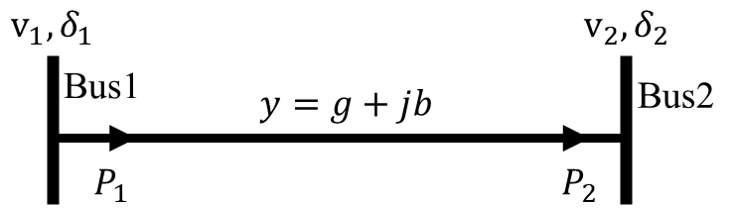
\includegraphics[width = 0.6\linewidth]{figs/A82/DC_PF.png}
\caption{Simple two bus system}
\label{fig:DC_PF}
\end{figure}

\subsection{Edge Cost Formulation}
The DC power-flow approximation in (\ref{eq:DC_PF_3}) is used to formulate the edge cost of the graph as a minimization problem which has a quadratic cost function and linear constraints. The cost function is shown in (\ref{eq:A2_CF}).
% The approximation used in (\ref{eq:DC_PF_3}) converts the non-linear AC power-flow equations into a linear equation. This facilitates formulating the equations to calculate the edge cost of the graph search problem as a quadratic program possible. Equation (\ref{eq:A2_CF}) shows the cost function.
\begin{multline}
\label{eq:A2_CF}
C_{total} = (P_{grid} * RTP + \sum_{n=1}^{N_{es}} (|P_{es}(n)|*r_{es}(n)) \\+
\sum_{m=1}^{N_{gen}}(A(m)*P_{gen}(m)^2 + B(m)*P_{gen}(m)))*\Delta T
\end{multline}
Here, $C_{total}$, $P_{grid}$ and $RTP$ represents the total cost of an edge, power drawn from the grid and the real-time price respectively.

 $N_{es}$ is the total number of energy storage in the system. $|P_{es}(n)$ is the power supplied by the $n^{th}$ energy storage. $r_{es}(n)$ is the levelized cost of using energy for the $n^{th}$ energy storage. $r_{es}(n)$ is calculated using (\ref{eq:R_ESS}). $N_{gen}$ is the total number of traditional generators in the system. $P_{gen}(m)$ is the power supplied by the $m^{th}$ generator. $A(m)$ and $B(m)$ are the constants used to calculate the operating cost of the $m^{th}$ generator \cite{saadat1999power}. The constant cost of operating a generator is ignored in this case as it is a constant cost and can not be reduced through optimization. $\Delta T$ signifies time in seconds between the parent and child node. The constraints of the cost function are defined by equations (\ref{eq:A2_EQ2}), and (\ref{eq:A2_EQ3}).
% \begin{equation}
% \label{eq:A2_EQ1}
% \sum_{n=1}^{N_{es}}P_{es}(n) + P_{grid} + \sum_{m=1}^{N_{gen}}P_{gen}(m) = \sum_{k=1}^{N_{load}}P_{load}(k) - \sum_{l=1}^{N_{PV}}P_{PV}(l)
% \end{equation}
% Here, $N_{load}$ is the total number of loads in the system. $P_{load}(k)$ is the power supplied by the $k^{th}$. $N_{PV}$ is the total number of PVs in the system, and 
\begin{equation}
\label{eq:A2_EQ2}
\sum_{n=1}^{N_{es}}P_{es}(n) = \Delta ES / \Delta T
\end{equation}
Equation (\ref{eq:A2_EQ2}) represents the equality constraints imposed by the graph search. As seen in Fig. \ref{fig:F1_1_Dis}, going from a parent node to a child node signifies a percentage change in the total energy storage capacity of the system. Here, $\Delta ES$ signifies the total change in energy required to match the percentage change in the total energy storage capacity determined by the graph edge. $\Delta ES$ is divided by $\Delta T$ to convert from energy to power. These constraints ensure that the power supplied or absorbed by the energy storage match the graph edge.
\begin{equation}
\label{eq:A2_EQ3}
P = P_{load} - P_{PV} - P_{es} = h*\Delta \delta 
\end{equation}
Equation (\ref{eq:A2_EQ3}) represents the equality constraints generated from DC power-flow. It is a matrix representation of (\ref{eq:DC_PF_3}) \cite{DC_PF1}. Here, $h$ is the admittance matrix of the system. $\Delta \delta$ is the matrix of angle difference between adjacent busses. The components of bus power vector P are:\\
$P_{load} =$ Power requirements of load.\\
$P_{PV} =$ Power supplied by PV.\\
$P_{es} =$ power supplied by es.\\


The inequality constants are expressed using equations (\ref{eq:A2_IEQ1}), (\ref{eq:A2_IEQ2}) and (\ref{eq:A2_IEQ3}).
\begin{equation}
\label{eq:A2_IEQ1}
0 \leq P_{gen}(m) \leq \overline{P_{gen}(m)}, \quad m = 1, 2, 3, ... , N_{gen}
\end{equation}
Equation (\ref{eq:A2_IEQ1}) represents the inequality constraints rising from the power limits of the traditional generators. $P_{gen}(m)$ is the power generated by the $m^{th}$ generator, and $\overline{P_{gen}(m)}$ is the upper limit of generation for the $m^{th}$ generator. $N_{gen}$ is the total number of generators available. This constraint ensures that all available generators in the system generates power within the operating limit of the respective generator.
\begin{multline}
\label{eq:A2_IEQ2}
\underline{ES(n)} \leq ES_{current}(n)+(P_{es}(n)*\Delta T) \leq \overline{ES(n)}, \\ n = 1, 2, 3, ... , N_{es}
\end{multline}
Equation (\ref{eq:A2_IEQ2}) represents the inequality constraints pertaining to the upper and lower state of energy bounds of energy storage. $\underline{ES(n)}$ is the lower bound of stored energy, and $\overline{ES(n)}$ is the upper bound of stored energy for the $n^{th}$ energy storage. $ES_{current}(n)$ is the energy stored in the energy storage at the parent node. $P_{es}(n)$ is the power supplied by the $n^{th}$ energy storage. A negative value for $P_{es}(n)$ signifies charging and a positive value signifies discharging. $P_{es}(n)$is multiplied by $\Delta T$ to convert it from power to energy.
\begin{equation}
\label{eq:A2_IEQ3}
\underline{P_{ES}(n)} \leq P_{es}(n) \leq \overline{P_{ES}(n)}, \quad n = 1, 2, 3, ... , N_{es}
\end{equation}
Equation (\ref{eq:A2_IEQ3}) shows the inequality constraints pertaining to the charging and discharging power rating of the energy storage. $\underline{P_{ES}(n)}$ is the highest charging power rating  and $\overline{P_{ES}(n)}$ is the highest discharging power rating of the $n^{th}$ energy storage. Equations (\ref{eq:A2_IEQ2}) and (\ref{eq:A2_IEQ3}) makes sure that all the energy storage in the system operate within their limits.

Combining all the equations from (\ref{eq:A2_CF}) to (\ref{eq:A2_IEQ3}) the full form of the quadratic programming formulation to solve the edge cost is as follows:\\
Minimize:
\begin{multline}
\label{eq:multi_all_in1}
(P_{grid} * RTP + \sum_{n=1}^{N_{es}} (|P_{es}(n)|*r_{es}(n)) + \\ \sum_{m=1}^{N_{gen}}(A(m)*P_{gen}(m)^2 + B(m)*P_{gen}(m)))*\Delta T
\end{multline}
Subject to:\\

$\sum_{n=1}^{N_{es}}P_{es}(n) = \Delta ES / \Delta T$

$P = P_{load} - P_{PV} - P_{es} = h*\Delta \delta $

$0 \leq P_{gen}(m) \leq \overline{P_{gen}(m)}$

$\underline{ES(n)} \leq ES_{current}(n)+(P_{es}(n)*\Delta T) \leq \overline{ES(n)}$

$\underline{P_{ES}(n)} \leq P_{es}(n) \leq \overline{P_{ES}(n)}$\\

Where,

$m = 1, 2, 3, ... , N_{gen}$, and $n = 1, 2, 3, ... , N_{es}$.\\

When calculating the $G_{cost}[child]$ of Algorithm 1, this minimization problem is solved to get the cost of the edges of the graph.
\subsection{Heuristic Cost Calculation}
The heuristic cost calculation function calculates the heuristic used by the A* search algorithm. In this case the heuristic cost is calculated using (\ref{eq:multi_hu1}).
\begin{equation}
\label{eq:multi_hu1}
    C_H(t) = \sum_{n=t}^{end} C_{best}(n)
\end{equation}

Here, $C_H(t)$ is the heuristic cost for time $t$ and $C_{best}(n)$ is the best possible cost at time $n$. The best possible cost is calculated by relaxing some of the constraints for (\ref{eq:multi_all_in1}). The cost function is kept the same. The constraints pertaining to energy storage availability from (\ref{eq:A2_IEQ2}) is removed. The constraint defined by (\ref{eq:A2_EQ2}) are also removed. The minimization problem solved to find $C_{best}(n)$ fot the time $n$ is as follows:\\
Minimize:
\begin{multline}
\label{eq:multi_hu2}
C_{best}(n)=(P_{grid} * RTP + \sum_{n=1}^{N_{es}} (|P_{es}(n)|*r_{es}(n)) +\\ \sum_{m=1}^{N_{gen}}(A(m)*P_{gen}(m)^2 + B(m)*P_{gen}(m)))*\Delta T
\end{multline}
Subject to:\\

$\sum_{n=1}^{N_{es}}P_{es}(n) = \Delta ES / \Delta T$


$0 \leq P_{gen}(m) \leq \overline{P_{gen}(m)}$


$\underline{P_{ES}(n)} \leq P_{es}(n) \leq \overline{P_{ES}(n)}$\\

Where,

$m = 1, 2, 3, ... , N_{gen}$, and $n = 1, 2, 3, ... , N_{es}$

\subsection{Using A* to Search the Graph}

\textbf{Algorithm 1:} A* search algorithm

\begin{algorithmic}[1]
\label{al:1}
% \Function{heuristic\_estimate}{$a,b$}
%     \State $hCost := \sum_{n=a}^b D(n)*R_{best}(n) $
%     \State \Return $hCost$
% \EndFunction

% \Function{gCost\_calc}{$p,c$}
%     \State $C_{actual}(pc) := C_{ESS}(pc)+C_{GRID}(t)+C_{best}(p)$
%     \State \Return $C_{actual}(pc)$
% \EndFunction

\Function{A*}{$start, goal$}
\State $Closed\_Set = \{\}$ \Comment{Set of evaluated nodes}
\State $Open\_Set = \{Start\}$ \Comment{Set of already discovered nodes which have not been evaluated. Initially,  the start node is discovered.}
\State $F\_cost[Start] = \infty$
\While{$Open\_Set$ is not empty}
    \State $Current\_Node = $ node in $Open\_Set$ with lowest $F\_cost$
    \If{$Current\_Node$ == goal}
      \State  \textbf{break} 
    \EndIf
    \For {Each child node of $Current\_Node$}
        \If{Child node in $Closed\_Set$}
            \State \textbf{continue}
        \EndIf
        \If{Child node in $Open\_Set$}
            \If{$G\_cost[child]$ $\geq$ $G\_cost$ already in $Open\_Set$}
                \State \textbf{continue}
            \EndIf
        \EndIf
        \State $Best\_Parent[child] = Current\_Node$
        \State $F\_cost[child] = G\_cost[child] + H\_cost[child]$
        \State $Open\_Set.add(child)$ \Comment{Add child node to $Open\_Set$}

    \EndFor
    \State $Closed\_Set.add(Current\_Node)$ \Comment{Add $Current\_Node$ to $Closed\_Set$}
    \State $Open\_Set.remove(Current\_Node)$ \Comment{Remove $Current\_Node$ From $Open\_Set$}
\EndWhile
\State $Best\_Path = \{ \}$ \Comment{$Best\_Path$ is the most efficient path to get to the goal node.}
\While{$Best\_Parent[Current\_Node] != Start$}
    \State $Current\_Node = Best\_Parent[Current\_Node]$
    \State $Best\_Path.add(Current\_Node)$ \Comment{Add $Current\_Node$ to $Best\_Path$}
\EndWhile
\State \Return $Best\_Path$
\EndFunction
\end{algorithmic}